\documentclass[dvipdfmx, 10pt]{beamer}
%%%% 和文用 %%%%%
\usepackage{bxdpx-beamer}
\usepackage{pxjahyper}
\usepackage{minijs}%和文用
\renewcommand{\kanjifamilydefault}{\gtdefault}%和文用
\usepackage{comment}

%%%%%%%%%%%%%%%%%%%%%%%%%%
%% usepackage 群
%%%%%%%%%%%%%%%%%%%%%%%%%%
\usepackage{amsmath,bm} %多次元空間ベクトルRを表記するのに必要
\usepackage{amsfonts}
\usepackage{ascmac} %枠付き文章を表記するのに必
\usepackage{amssymb}
%\usepackage[dvipdfmx]{animate}
%\usepackage[dvipdfmx]{graphicx}
% \mathbb{R}^{l} %表記例
% \usepackage{algorithm}
% \usepackage{algorithmicx}
% \usepackage{algpseudocode}

%%%% スライドの見た目 %%%%%
\usetheme{metropolis}
\usefonttheme{professionalfonts}

%%%% metropolisの設定 %%%%%
\metroset{block=fill}


%\useoutertheme[subsection=false]{smoothbars}%ヘッダーにセクション表示
\useinnertheme{circles} % 箇条書きをシンプルに

\setbeamercovered{transparent}%消えている文字をうっすらと表示
\setbeamertemplate{footline}[frame number]%フッターをページ番号だけに
\setbeamerfont{footline}{size=\scriptsize}%ページ番号小さく
\setbeamerfont{frametitle}{size=\large}%フレームタイトルちょい小さく
\setbeamercolor{footline}{bg=black}%ページ番号を太く
\setbeamersize{text margin left=.75zw, text margin right=.75zw}%スライドの横の空白を調節

\setbeamertemplate{enumerate items}[default]%enumerate環境のitemを見やすくする
\setbeamertemplate{section in toc}[square]%outlineのボールを四角に
\setbeamertemplate{navigation symbols}{}%右下のアイコンを消す

% blockの色定義
\definecolor{BlueTOL}{HTML}{222255}
\definecolor{BrownTOL}{HTML}{666633}
\definecolor{GreenTOL}{HTML}{225522}

\setbeamercolor{block title alerted}{fg=BrownTOL}
\setbeamercolor{block title example}{fg=GreenTOL}

%%%%

%%%%%%%%%%%%%%%%%%%%%%%%%%%%%%%%%%%%%%%%%%%%
%%いろいろ便利なもの
%%%%%%%%%%%%%%%%%%%%%%%%%%%%%%%%%%%%%%%%%%%%
\usepackage{here} %[hbtp]の代わりに[H]と書きこむと強制的にその場所に図や表を挿入する
\usepackage{bm}

%%%%%%%%%%%%%%%%%%%%%%%%%%%%%%%%%%%%%%%%%%%%%%%%%
%%newcommand群
%%%%%%%%%%%%%%%%%%%%%%%%%%%%%%%%%%%%%%%%%%%%%%%%%
\newcommand{\argmax}{\mathop{\rm arg~max}\limits}
\newcommand{\argmin}{\mathop{\rm arg~min}\limits}

\newcommand{\x}{\mbox{\boldmath$x$}}
\newcommand{\y}{\mbox{\boldmath$y$}}
%%%%%%%%%%%%%%%%%%%%%%%%%%%%%%%%%%%%%%%%%%%%%%%%%
%%本文
%%%%%%%%%%%%%%%%%%%%%%%%%%%%%%%%%%%%%%%%%%%%%%%%%
\title[]{DeepLearninig 勉強会}
\author[T.Ochiai]{B4 T.Ochiai}
\date[\today]{\today}
\institute[NIT]{Nagoya Institute of Technology \\ Takeuchi \& Karasuyama Lab}
% [..]に省略名が書ける

%目次スライド
\AtBeginSection[]{
    \begin{frame}{Next Section}
	\tableofcontents[currentsection, hidesubsections]%目次本体
	%\thispagestyle{empty}%ヘッダーフッター表示なし
	\end{frame}
}

\begin{document}

%-------------------

%タイトル
\begin{frame}[plain]
\titlepage
\end{frame}

%-------------------

%目次
\begin{frame}{目次}
\tableofcontents[hideallsubsections]
\end{frame}

%-------------------

\section{はじめに}

%-------------------

\begin{frame}{Deep Learningについて}
  \begin{itemize}
    \item 機械学習の一種
    \begin{itemize}
      \item 機械学習の基礎を理解する必要がある
    \end{itemize}
  \end{itemize}
  \centering 今回は機械学習の\textcolor{red}{基礎}についてお話しします
\end{frame}

%-------------------

\section{学習アルゴリズム}

%-------------------

\begin{frame}{学習アルゴリズムについて}
  \begin{itemize}
    \item 機械学習はデータを元にして学習を行う
    \item ここでの学習とは何か?
    \begin{itemize}
      \item experiences $E$
      \item tasks $T$
      \item performance measures $P$
    \end{itemize}
  \end{itemize}
\end{frame}

%-------------------

\begin{frame}{タスク $T$}
  \begin{itemize}
    \item 機械学習は人間界において解決するのが難しいタスクを解決する
    \begin{itemize}
      \item 学習過程自体がタスクではない
      \item 例: ロボットを歩かせるための学習では「歩かせる」ことがタスクである
    \end{itemize}
    \item 標本をどのような過程で処理するかという面で説明される
    \begin{itemize}
      \item 標本とは\textcolor{red}{特徴}の集合である
      \item 標本はよく$\bm{x} \in \mathbb{R} ^ {n}$で表す
    \end{itemize}
    \item 機械学習ではたくさんのタスクを解くことができる
  \end{itemize}
\end{frame}

%-------------------

\begin{frame}{Classification}
  \begin{itemize}
    \item $k$個のカテゴリの中のどれに所属するのかを決定
    \begin{itemize}
      \item 関数$f: \mathbb{R} ^ {n} \to \{1, ..., k\}$を学習
      \item $y = f(\bm{x})$において$\bm{x}$は標本ベクトル , $y$はカテゴリに対応する数値
    \end{itemize}
  \end{itemize}
  \begin{exampleblock}{例}
    \begin{itemize}
      \item 画像の分類
      \begin{itemize}
        \item $\bm{x}$ : 画像
        \item $y$ : 画像のカテゴリを識別するラベル
      \end{itemize}
    \end{itemize}
    \begin{itemize}
      \item 撮った写真を自動でタグ付けしたりする技術など
    \end{itemize}
  \end{exampleblock}
\end{frame}

%-------------------

\begin{frame}{Classification with missing inputs}
  \begin{itemize}
    \item 入力に欠損データがあるときのClassification
    \item 1つの関数を学習するより複数の関数の集合を学習する方がよい
    \item 最大で$2 ^ {n}$個の関数を考えれば解決できる
  \end{itemize}
\end{frame}

%-------------------

\begin{frame}{Regression}
  \begin{itemize}
    \item 入力に対してある数値を予測する
    \begin{itemize}
      \item 関数$f: \mathbb{R} ^ {n} \to \mathbb{R}$を学習
    \end{itemize}
    \item 出力がラベルではないこと以外はClassificationと同じ
  \end{itemize}
  \begin{exampleblock}{例}
    \begin{itemize}
      \item 被保険者が支払う額の予測
      \item 証券の将来の価格の予測
    \end{itemize}
  \end{exampleblock}
\end{frame}

%-------------------

\begin{frame}{Transcription}
  \begin{itemize}
    \item 非構造化されたデータをテキストデータに変換する
  \end{itemize}
  \begin{exampleblock}{例}
    \begin{itemize}
      \item 画像中の文字の認識
      \begin{itemize}
        \item $\bm{x}$ : あるテキストを含んだ画像
        \item $y$ : 画像中に含まれているテキスト
      \end{itemize}
      \item スピーチの認識
      \begin{itemize}
        \item $\bm{x}$ : ある文字列が話されたときの音波の波形
        \item $y$ : 実際に話された文字列
      \end{itemize}
    \end{itemize}
  \end{exampleblock}
\end{frame}

%-------------------

\begin{frame}{Machine translation}
  \begin{itemize}
    \item ある言語を他の言語に翻訳する
    \item 自然言語に用いることが可能
  \end{itemize}
\end{frame}

%-------------------

\begin{frame}{Structured output}
  \begin{itemize}
    \item 出力がベクトルであるようなタスク全般
    \begin{itemize}
      \item または出力が複数個の値であるタスク
    \end{itemize}
  \end{itemize}
  \begin{exampleblock}{例}
    \begin{itemize}
      \item 自然言語の品詞へのパース
      \item 画像内の各ピクセルをあるカテゴリに分類するタスク
    \end{itemize}
  \end{exampleblock}
\end{frame}

%-------------------

\begin{frame}{Anomaly detection}
  \begin{itemize}
    \item ある物事が正常か異常かを検知するタスク
  \end{itemize}
  \begin{exampleblock}{例}
    \begin{itemize}
      \item クレジットカード詐欺の検知
      \begin{itemize}
        \item 普段とは違うタイプの買い物がなされたときに対して異常検知を行う
        \item 異常が検知された場合はクレジットカードの利用を止めて詐欺を防ぐことができる
      \end{itemize}
    \end{itemize}
  \end{exampleblock}
\end{frame}

%-------------------

\begin{frame}{Synthesis and sampling}
  \begin{itemize}
    \item 訓練データ元に新たな標本をサンプリングする
    \item 入力が与えられたときサンプリングやその合成手順によって出力を生成する
    \item ある入力に対しての正しい出力は存在しない
    \begin{itemize}
      \item 複数のパターンの出力
    \end{itemize}
  \end{itemize}
  \begin{exampleblock}{例}
    \begin{itemize}
      \item ゲームにおけるテクスチャや地形の自動生成
      \item 文章からその文章を読み上げるオーディオ波形の生成
    \end{itemize}
  \end{exampleblock}
\end{frame}

%-------------------

\begin{frame}{Imputation of missing values}
  \begin{itemize}
    \item 入力データ中の欠損値の補完
  \end{itemize}
\end{frame}

%-------------------

\begin{frame}{Denoising}
  \begin{itemize}
    \item 入力に含まれるノイズを除去する
    \item ノイズの含まれる入力 $\tilde{\bm{x}} \in \mathbb{R}$
    \item ノイズを除去した入力 $\bm{x} \in \mathbb{R}$
    \item 一般的には予測分布 $p(\bm{x}|\tilde{\bm{x}})$ を求める
  \end{itemize}
\end{frame}

%-------------------

\begin{frame}{Density estimation}
  \begin{itemize}
    \item 関数 $p_{model} : \mathbb{R} ^ {n} \to \mathbb{R}$ を学習する
    \begin{itemize}
      \item $p_{model}$は確率密度関数であると解釈できる
    \end{itemize}
    \item 分布を捉えることができる
    \item 欠損データにも用いることができる
    \begin{itemize}
      \item $i$番目の特徴が欠損している$\bm{x}_{-i}$
      \item $p(x_{i}|\bm{x_{-1}})$を考えることで欠損データにも対応可能
    \end{itemize}
  \end{itemize}
\end{frame}

%-------------------

\begin{frame}{The Performance Measure $P$}
  \begin{itemize}
    \item 機械学習アルゴリズムの性能を定量的に計測する必要がある
    \begin{itemize}
      \item accuracy
      \item error rate
    \end{itemize}
    \item 実際は未知のデータに対する機械学習アルゴリズムの性能を計測したい
    \begin{itemize}
      \item training data で学習を行い {\bf test data} で未知データへの性能を評価
    \end{itemize}
    \item 問題設定にあった性能指標を見つけるのは実際難しい
    \begin{itemize}
      \item 何を計測するべきかを決めるのが難しい
      \item タスクによって異なる指標を選択する必要がある
    \end{itemize}
  \end{itemize}
\end{frame}

%-------------------

\begin{frame}{The Experience, $E$}
  \begin{itemize}
    \item 機械学習アルゴリズムは2つの種類に分けることができる
      \begin{itemize}
        \item 教師なし学習
        \item 教師あり学習
      \end{itemize}
    \item 機械学習アルゴリズムは\textcolor{red}{データセット}をもとに学習を行う
    \item データセットは標本の集合で\textcolor{red}{データ点}とも呼ぶ
  \end{itemize}
\end{frame}

%-------------------

\begin{frame}{Unsupervised learning algorithms}
  \begin{itemize}
    \item データセットの構造の特性を学習する
    \begin{itemize}
      \item 厳密にはデータセットを生成した確率分布を学習
    \end{itemize}
    \begin{exampleblock}{例}
      \begin{itemize}
        \item 密度推定
        \item ノイズ除去
        \item クラスタリング
      \end{itemize}
    \end{exampleblock}
  \end{itemize}
\end{frame}

%-------------------

\begin{frame}{Supervised learning algorithms}
  \begin{itemize}
    \item 教師なし学習とは違い訓練データに{\bf label}が含まれる
    \begin{itemize}
      \item labelは{\bf target}とも呼ばれる
    \end{itemize}
    \item 入力: $\bm{x}$,label: $y$を用いて$\bm{x}$から$y$を予測できるように学習を行う
  \end{itemize}
  \begin{exampleblock}{Irisデータセットの例}
    \begin{itemize}
      \item $\bm{x}$はあやめのいくつかの特徴
      \item $y$はあやめの種類を表すコード
    \end{itemize}
  \end{exampleblock}
\end{frame}

%-------------------

\begin{frame}{教師あり学習,教師なし学習,その他の学習}
  \begin{itemize}
    \item 教師あり学習と教師なし学習は大まかに適応すべきケースが決まっている
    \item 教師あり学習
    \begin{itemize}
      \item 回帰
      \item クラス分類
      \item structured output problems
    \end{itemize}
    \item 教師なし学習
    \begin{itemize}
      \item Density estimation
    \end{itemize}
    \item そのほかにもいくつかの学習が存在する
    \begin{itemize}
      \item semi supervised learning
      \begin{itemize}
        \item いくつかの標本にのみlabelが存在する
      \end{itemize}
      \item multi-instance learning
      \begin{itemize}
        \item labelを含む,含まないという情報のみは与えられるがlabelの値はわからない
      \end{itemize}
    \end{itemize}
  \end{itemize}
\end{frame}

%-------------------

\begin{frame}{計画行列}
  \begin{itemize}
    \item ほとんどの機械学習アルゴリズムでは標本の集合を用いて学習を行う
    \item 標本の集合は通常,計画行列として表わされる
    \begin{itemize}
      \item 計画行列は各行に各標本,各列に各特徴をもつ
      \item 各行に同じサイズの標本ベクトルをもつような行列であると考えてもよい
    \end{itemize}
  \item 教師あり学習では計画行列は$\bm{X}$,ラベルは$\bm{y}$として表されることが多い
  \begin{itemize}
    \item $y_{i}$は$i$番目の標本のラベル
  \end{itemize}
  \end{itemize}
\end{frame}

%-------------------

\section{線形回帰}

%-------------------
\begin{frame}{線形回帰}
  \begin{itemize}
    \item 入力$\bm{x} \in \mathbb{R} ^ {n}$から出力$y \in \mathbb{R}$を予測する
    \item 予測値を$\hat{y}$ , $\bm{w}$を重みパラメータとして以下のような回帰問題を考える
    \begin{itemize}
      \item $\bm{w}$は$\bm{x}$の各要素に対する重み
      \item $w_{i}$の絶対値が大きいほど$x_{i}$が回帰の結果に強く寄与する
    \end{itemize}
  \end{itemize}
  \begin{equation}
    \hat{y} = \bm{w} ^ {\top} \bm{x}
  \end{equation}
  \begin{itemize}
    \item $\bm{w}$を訓練データによって学習することを目指す
  \end{itemize}
\end{frame}

%-------------------

\begin{frame}{Mean Squared Error}
  \begin{itemize}
    \item 線形回帰の性能指標として{\bf Mean Squared Error} (MSE)を用いる
    \item テストデータの計画行列を$\bm{X} ^ {(test)}$ , targetsを$\bm{y} ^ {(test)}$ , 予測値を$\hat{\bm{y}} ^ {(test)}$としてテストデータにおける$MSE_{test}$は以下のように表される
  \end{itemize}
  \begin{equation}
    MSE_{test} = \dfrac{1} {m} \| \hat{\bm{y}} ^ {(test)} - \bm{y} ^ {(test)} \| _{2}^{2}
  \end{equation}
  \begin{itemize}
    \item targetsと予測値の距離が遠いほど$MSE_{test}$の値は大きくなる
    \item $MSE_{test}$の値を可能な限り\textcolor{blue}{小さく}したい
    \begin{itemize}
      \item targetsと予測値を近くしたい
    \end{itemize}
  \end{itemize}
\end{frame}

%-------------------

\begin{frame}{MSEによるパラメータの最適化}
  \begin{itemize}
    \item 訓練データ$(\bm{X}_{train}, \bm{y}_{train})$を用いて線形回帰モデルを学習する
    \item $MSE_{train}$を最小にするような$\bm{w}$を求める
    \begin{itemize}
      \item $MSE_{train}$を$\bm{w}$で微分してその値(勾配)が$\bm{0}$となる$\bm{w}$を求める
    \end{itemize}
  \end{itemize}
  \begin{gather}
    \dfrac{\partial} {\partial \bm{w}} MSE_{train} = 0 \\
    \dfrac{\partial} {\partial \bm{w}} \dfrac{1} {m}\| \hat{\bm{y}} ^ {(train)} - \bm{y} ^ {(train)} \| _{2}^{2} = 0 \\
    \dfrac{1} {m} \dfrac{\partial} {\partial \bm{w}} \| \bm{X}^{(train)} \bm{w} - \bm{y} ^ {(train)} \| _{2}^{2} = 0 \\
    ..... \nonumber \\ 
    \bm{w} = (\bm{X} ^ {(train)\top} \bm{X} ^ {(train)}) ^ {-1} \bm{X} ^ {(train)\top} \bm{y} ^ {(train)}
  \end{gather}
  \begin{itemize}
    \item 式(6)の方程式のことを一般に\textcolor{red}{正規方程式}と呼ぶ
  \end{itemize}
\end{frame}

%-------------------

\begin{frame}{MSEによるパラメータの最適化の例}
  \begin{figure}[htbp]
     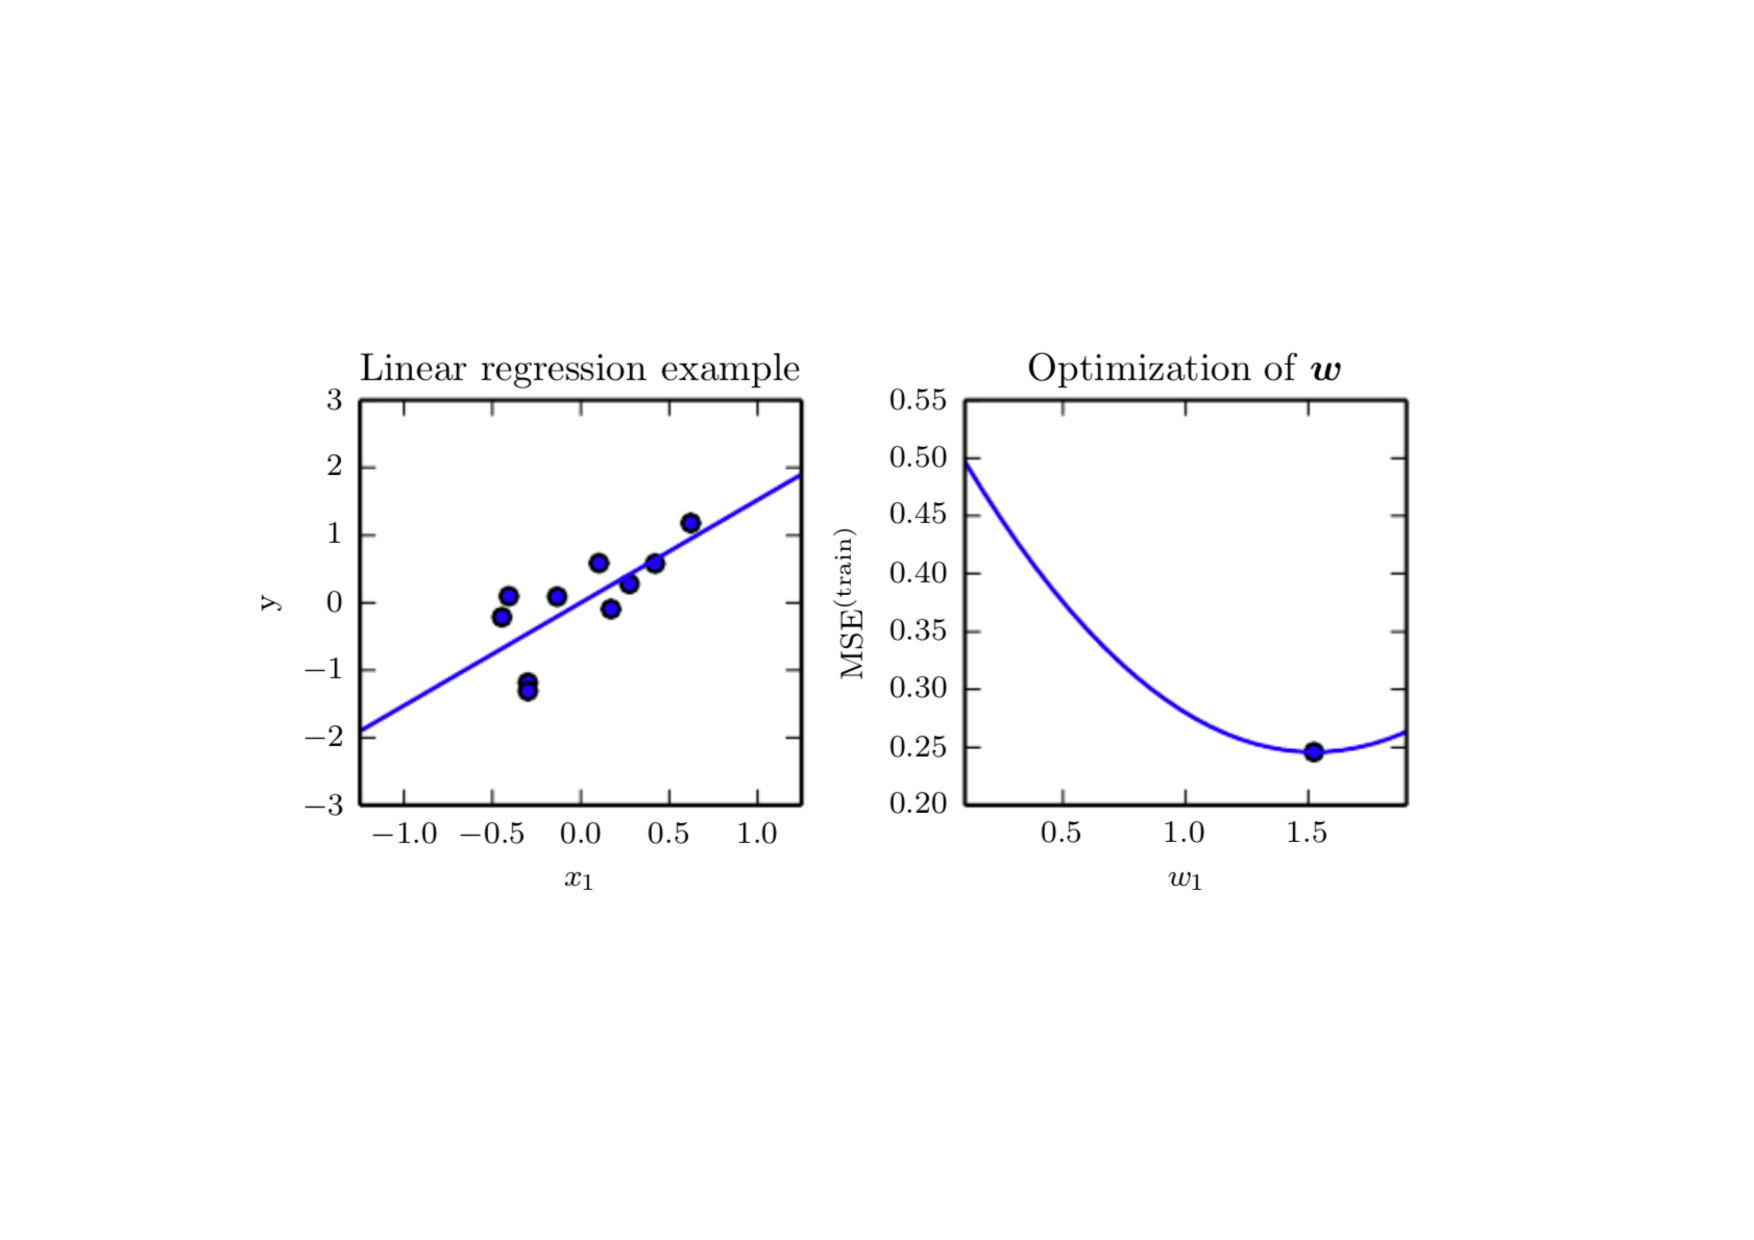
\includegraphics[keepaspectratio, scale=0.4, angle=-90]{./images/mse-opt.pdf}
     \caption{$\bm{w}$の最適化の結果}
  \end{figure}
  \begin{itemize}
    \item 最適化によって訓練データ点をうまく直線回帰できている
  \end{itemize}
\end{frame}

%-------------------

\begin{frame}{バイアス項を含む線形回帰}
  \begin{itemize}
    \item 一般に線形回帰を考えるときは上述の線形モデル対してさらに\textcolor{red}{バイアス項} $b$ を考慮したモデルを考えることが多い
  \end{itemize}
  \begin{equation}
    \hat{y} = \bm{w} ^ {\top} \bm{x} + b
  \end{equation}
  \begin{itemize}
    \item 入力が全くない場合にモデルの出力が$b$に偏るという観点に由来する
    \item 統計的バイアスの考えとは異なることに注意
  \end{itemize}
\end{frame}

%-------------------

\section{容量,過学習,未学習}

%-------------------

\begin{frame}{汎化性能}
  \begin{itemize}
    \item 機械学習では未知の入力に対しての\textcolor{red}{汎化性能}が重要
    \item モデルを学習させるためには\textcolor{red}{訓練誤差}を小さくする
    \begin{itemize}
      \item これだけならば単なる最適化問題
    \end{itemize}
    \item 機械学習が最適化問題と異なるのは学習したモデルでテスト誤差も小さくしたい点
    \begin{itemize}
      \item テスト誤差 : $\dfrac{1} {m} \| \bm{X} ^ {(test)\top} \bm{w} - \bm{y} ^ {(test)} \| _{2}^{2}$
    \end{itemize}
  \end{itemize}
\end{frame}

%-------------------

\begin{frame}{i.i.d.仮定}
  \begin{itemize}
    \item 訓練データとテストデータは\textcolor{red}{データ生成過程}と呼ばれるデータ集合の確率分布から生成される
    \item 通常は\textcolor{red}{i.i.d.仮定}という仮定を置く
    \begin{itemize}
      \item 各データ集合が互いに独立
      \item 訓練集合とテスト集合が同一の分布にしたがう
    \end{itemize}
    \item 仮定をおくことで訓練誤差とテスト誤差の関係を数学的に調べることが可能
    \begin{itemize}
      \item 無作為に選択されたモデルの期待訓練誤差と期待テスト誤差が等しい
    \end{itemize}
  \end{itemize}
\end{frame}

%-------------------

\begin{frame}{過学習と未学習}
  \begin{itemize}
    \item 機械学習がどの程度うまく動作するかには以下の要素がある
    \begin{itemize}
      \item 訓練誤差を小さくする
      \item 訓練誤差とテスト誤差の差を小さくする
    \end{itemize}
    \item これら2つの要素は\textcolor{red}{過学習} , \textcolor{blue}{未学習}に対応する
    \begin{itemize}
      \item 訓練集合で十分小さな誤差が得られない $\to$ 未学習
      \item 訓練誤差とテスト誤差の差が大きすぎる $\to$ 過学習
    \end{itemize}
  \end{itemize}
\end{frame}

%-------------------

\begin{frame}{モデルの容量}
  \begin{itemize}
    \item 過学習や未学習を起こしやすいかどうかはモデルの\textcolor{red}{容量}で制御できる
    \begin{itemize}
      \item 容量が小さい場合は訓練集合を適合させにくい
      \item 容量が大きい場合は訓練集合の特徴を記憶し過ぎてしまう
    \end{itemize}
    \item タスクの複雑さと訓練データの量に対して適切な容量があるときに最もよい性能を発揮する

    \item モデルの容量を変更する方法
    \begin{itemize}
      \item \textcolor{red}{仮説空間}を選ぶ
      \item 入力される特徴量の数を変更し,対応するパラメータを追加する
    \end{itemize}
  \end{itemize}
\end{frame}

%-------------------

\begin{frame}{過学習と未学習の例}
  \begin{figure}[htbp]
     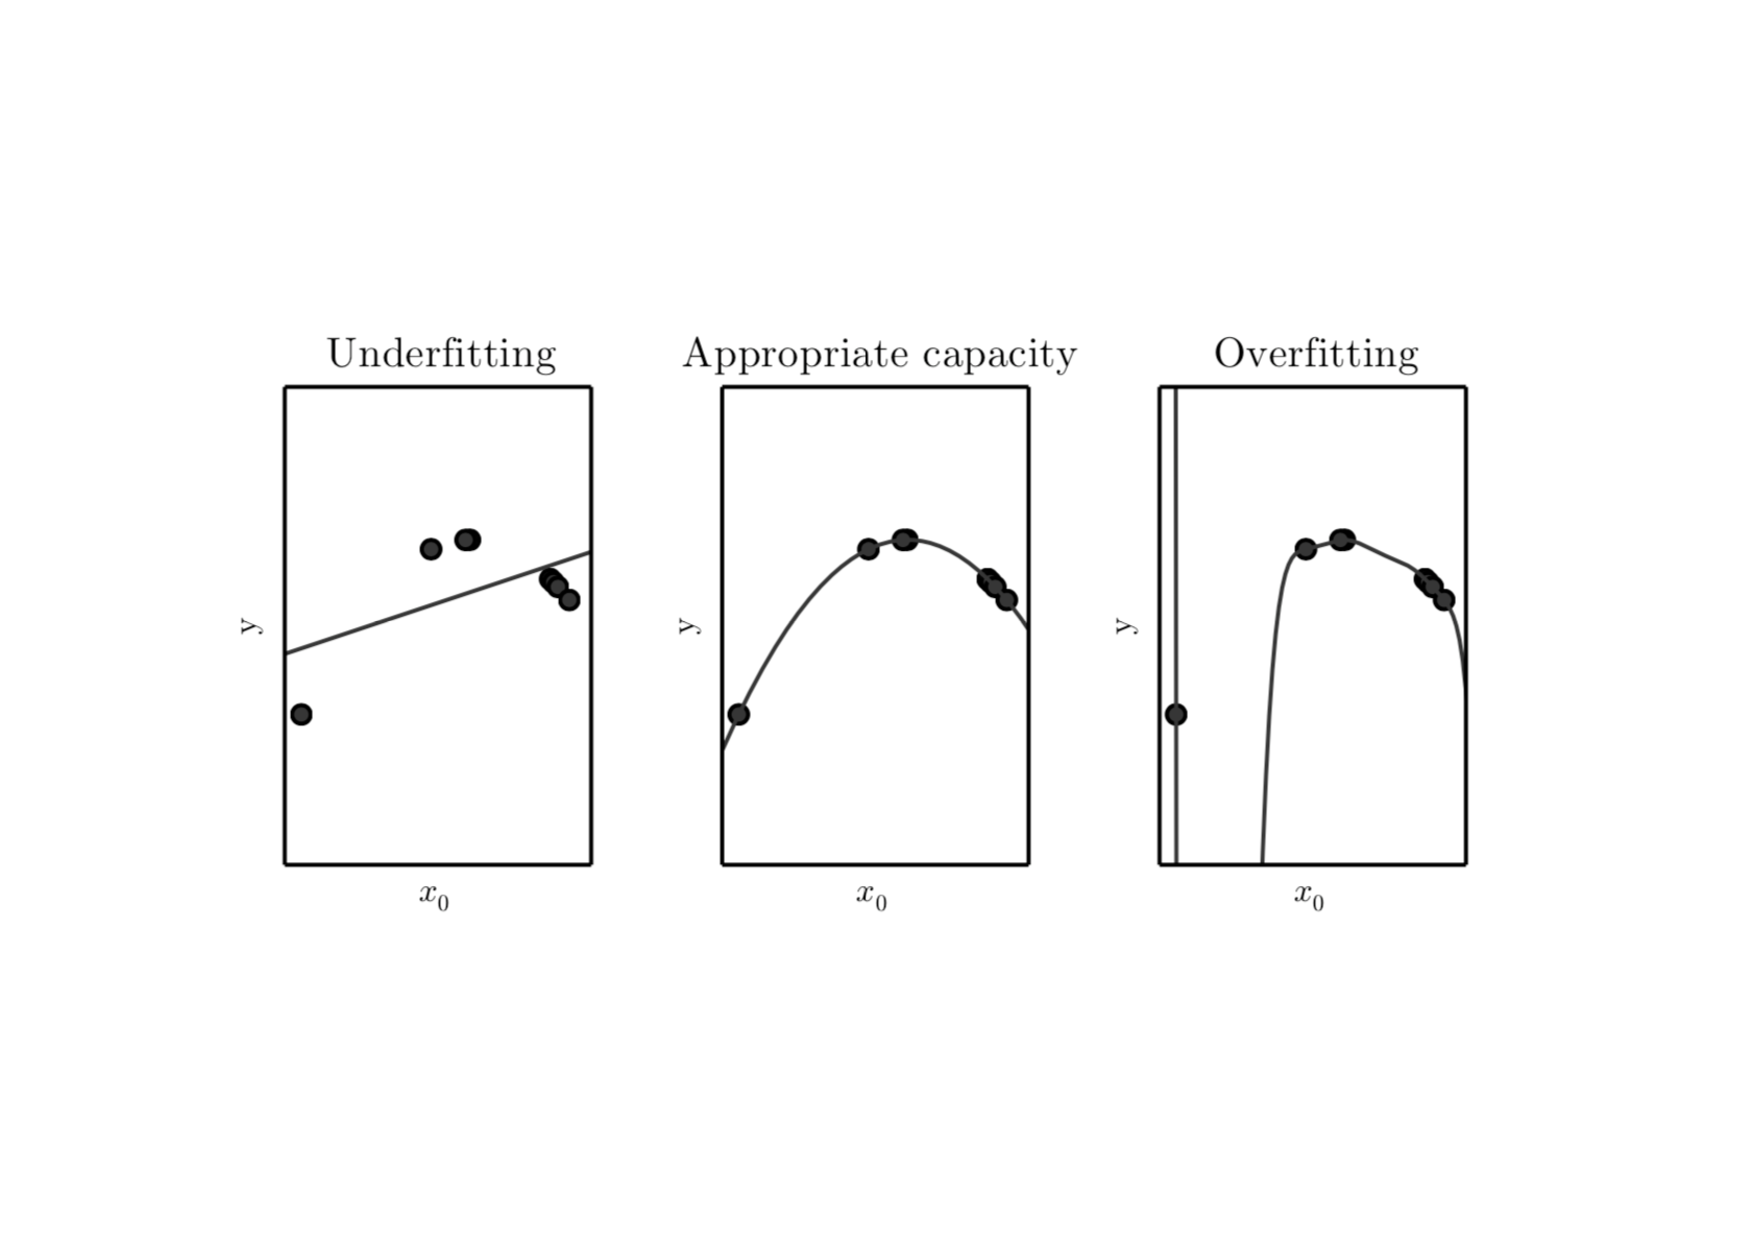
\includegraphics[keepaspectratio, scale=0.4, angle=-90]{./images/over-under-fitting.pdf}
     \caption{真の関数が2次であるような問題に対して(左) 線形 , (真ん中) 2次 , (右) 9次 の予測モデルで回帰した結果}
  \end{figure}
  \begin{itemize}
    \item 線形モデルの場合は容量が小さく未学習
    \item 9次の場合は容量が大きすぎるため過学習
  \end{itemize}
\end{frame}

%-------------------

\begin{frame}{オッカムの剃刀}
  \begin{itemize}
    \item 競合する複数の仮説が既知の観察を同様にうまく行える場合,「最も単純な」仮説を選ぶべき
    \begin{itemize}
      \item 同様の性能が得られるならば最も容量の小さいモデルを選択すべき
    \end{itemize}
    \item モデルの容量を定量化する方法として\textcolor{red}{VC次元}がある
    \begin{itemize}
      \item 二項分類の容量を測る
    \end{itemize}
    \item 訓練誤差とテスト誤差の差はモデルの容量が増えるほど大きくなる
    \begin{itemize}
      \item 容量が定量化できると定量的な予測を行うことが可能となる
    \end{itemize}
    \item 任意の高い容量というモデルを選ぶならばノンパラメトリックを選べばよい
  \end{itemize}
\end{frame}

%-------------------

\begin{frame}{容量と誤差との関係}
  \begin{figure}[htbp]
     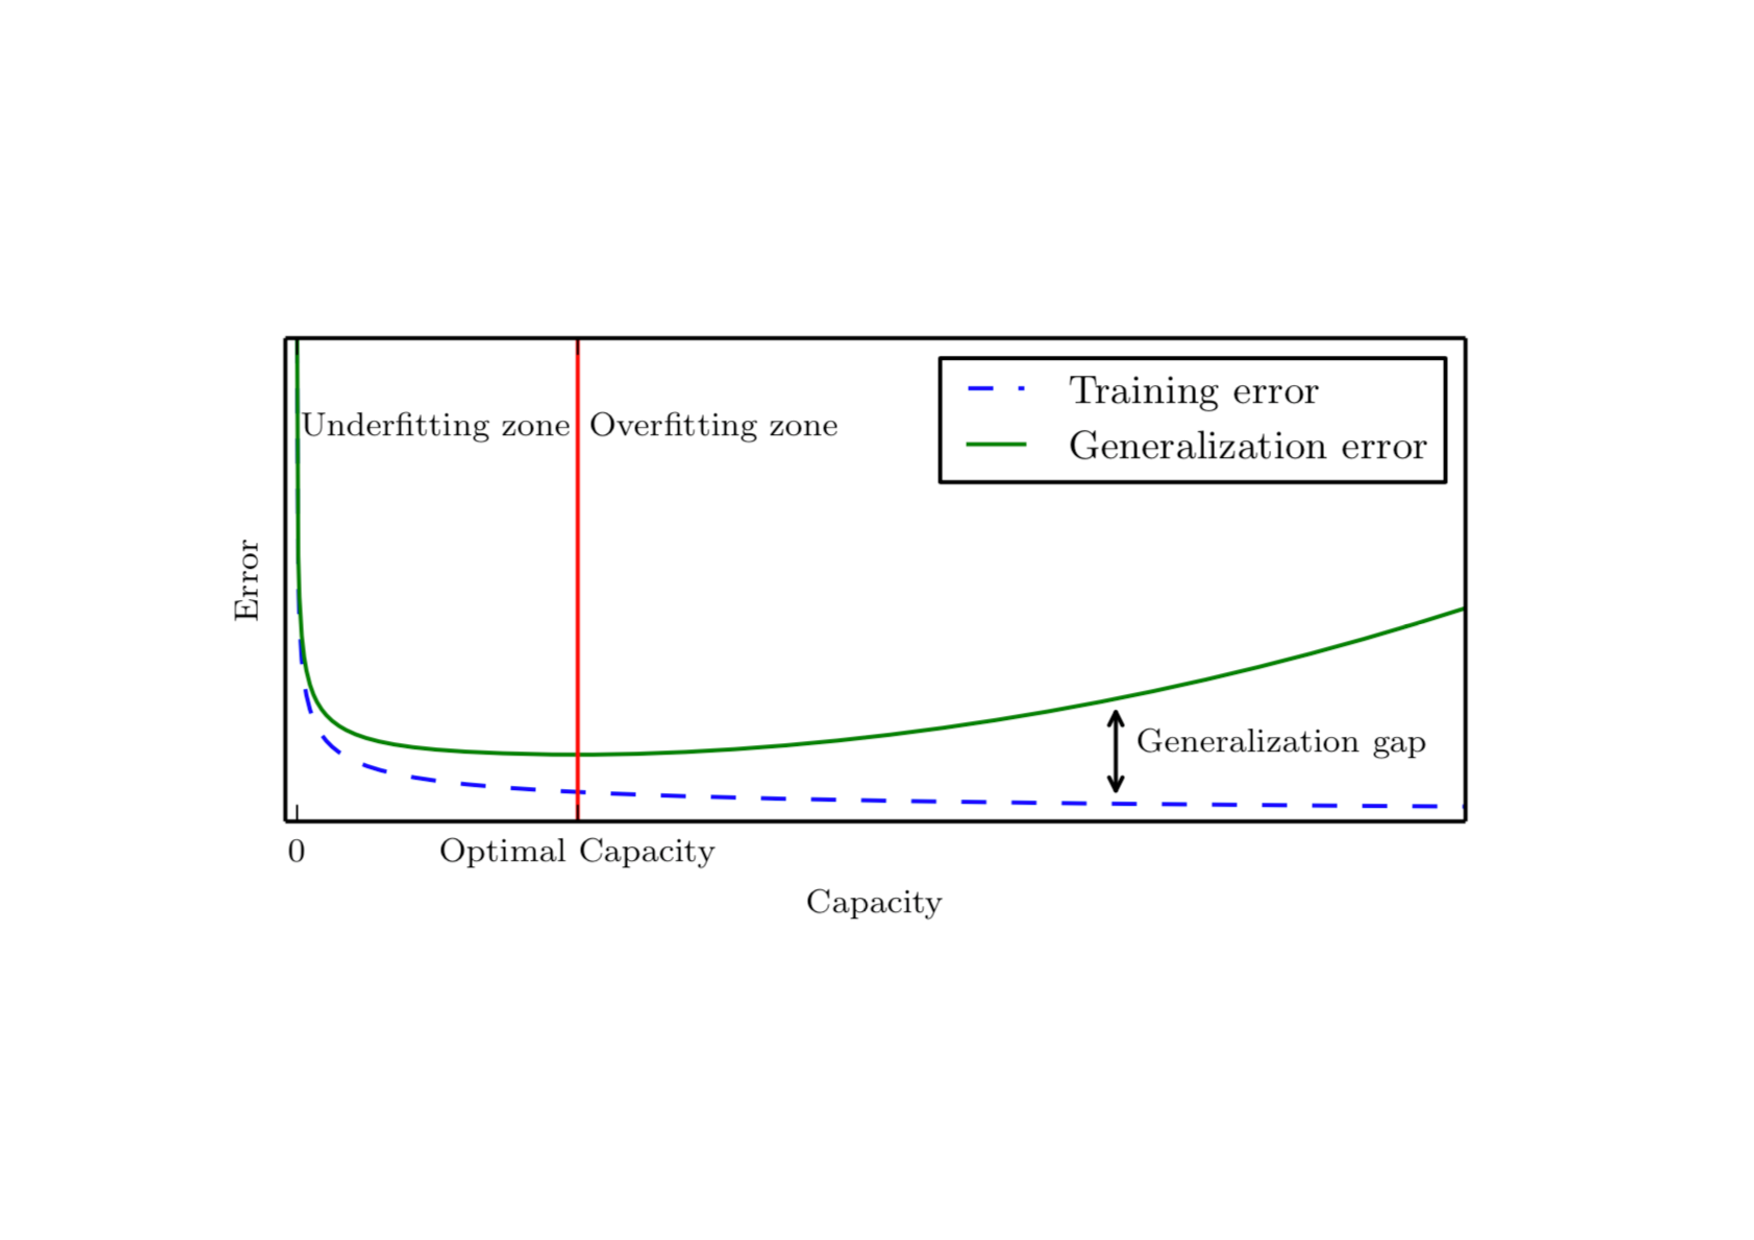
\includegraphics[keepaspectratio, scale=0.4, angle=-90]{./images/capacity.pdf}
     \caption{容量と誤差の関係.青点線は訓練誤差 , 緑実線はテスト誤差 , 赤線の位置は最適な容量}
  \end{figure}
  \begin{itemize}
    \item 最適な容量になるまでは未学習の状態
    \item 最適な容量を超えると各誤差の差が大きくなり過学習の状態
  \end{itemize}
\end{frame}

%-------------------

\begin{frame}{ノーフリーランチ定理}
  \begin{itemize}
    \item データを生成する分布全てを平均すると,どの分類アルゴリズムも平均すると未知のデータに対する誤差率は同じになる
    \item 他の機械学習アルゴリズムよりも普遍的に良いと呼ばれるアルゴリズムはないと言われている
    \begin{itemize}
      \item \textcolor{red}{ノーフリーランチ定理}という
    \end{itemize}
    \item データを生成する\textcolor{red}{すべての}分布を平均化した場合にのみ成立する
    \begin{itemize}
      \item 実世界の応用で出現する確率分布の種類に仮定を設けることでその分布に対して良い性能を発揮するアルゴリズムを設計できる
    \end{itemize}
  \end{itemize}
\end{frame}

%-------------------

\begin{frame}{正則化}
  \begin{itemize}
    \item 仮説空間内のある解を他の解より優先させることが可能
    \item 例えば以下のような\textcolor{red}{重み減衰}によって重みパラメータの訓練基準を変更することができる
  \end{itemize}
  \begin{equation}
    J(\bm{w}) = MSE_{train} + \lambda \bm{w}^{\top} \bm{w}
  \end{equation}
  \begin{itemize}
    \item $\lambda$が大きいほど重みパラメータは小さくなる
    \item 重み減衰によって未学習や過学習の傾向を制御することができる
    \item 一般には\textcolor{red}{正則化項}というペナルティをコスト関数に加えてモデルを\textcolor{red}{正則化}できる
    \item 正則化は訓練誤差ではなく汎化誤差を減少させる目的でアルゴリズムに変更を加える
  \end{itemize}
\end{frame}

%-------------------

\section{ハイパーパラメータと検証集合}

%-------------------

\begin{frame}{ハイパーパラメータ}
  \begin{itemize}
    \item ほとんどの機械学習アルゴリズムにはその挙動を制御する\textcolor{red}{ハイパーパラメータ}という設定値がある
    \item ハイパーパラメータは学習によって最適化はされない
    \begin{itemize}
      \item 訓練集合によって学習されたハイパーパラメータは常に最大のモデル容量を選択するため過学習を起こす
    \end{itemize}
  \end{itemize}
\end{frame}

%-------------------

\begin{frame}{検証集合}
  \begin{itemize}
    \item ハイパーパラメータを決定するためには\textcolor{red}{検証集合}を用いる
    \item 検証集合は訓練データの一部から構築される
    \begin{itemize}
      \item 訓練データを2つの別々のセットに分割する
      \item 分割されたセットの1つでパラメータの学習を行う
      \item もう片方のセットを検証集合として用いて汎化誤差の推定に用いる
      \item 汎化誤差に応じてパラメータを更新する
    \end{itemize}
    \item テスト集合は検証集合に用いてはいけない
    \begin{itemize}
      \item 学習にテスト集合を用いてはいけないのと同様
    \end{itemize}
    \item 検証集合を用いると汎化誤差は過小評価される
    \begin{itemize}
      \item 訓練誤差よりはその度合いは小さい
    \end{itemize}
  \end{itemize}
\end{frame}

%-------------------

\begin{frame}{交差検証}
  \begin{itemize}
    \item データ集合を訓練集合とテスト集合に分割するとテスト集合が小さくなったときに問題が生じる可能性がある
    \begin{itemize}
      \item 平均テスト誤差に対する不確実性が大きくなり,アルゴリズムの性能の比較が難しくなる
    \end{itemize}
    \item 無作為に訓練集合とテスト集合を分割して性能を評価することを繰り返すことですべてのデータにおいて平均テスト誤差を評価できる
    \begin{itemize}
      \item このような方法を\textcolor{red}{交差検証}と呼ぶ
    \end{itemize}
  \item 一般的なものとして\textcolor{red}{k-分割交差検証法}がある
  \end{itemize}
\end{frame}

%-------------------

\begin{frame}{k-分割交差検証法の例}
  % https://www.google.com/search?q=k-fold+%E4%BA%A4%E5%B7%AE%E6%A4%9C%E8%A8%BC&source=lnms&tbm=isch&sa=X&ved=0ahUKEwik_dfu45PiAhW3wosBHXbuCboQ_AUIDygC&biw=1440&bih=765#imgrc=ivj2nG0boYex-M:
  \begin{figure}[htbp]
     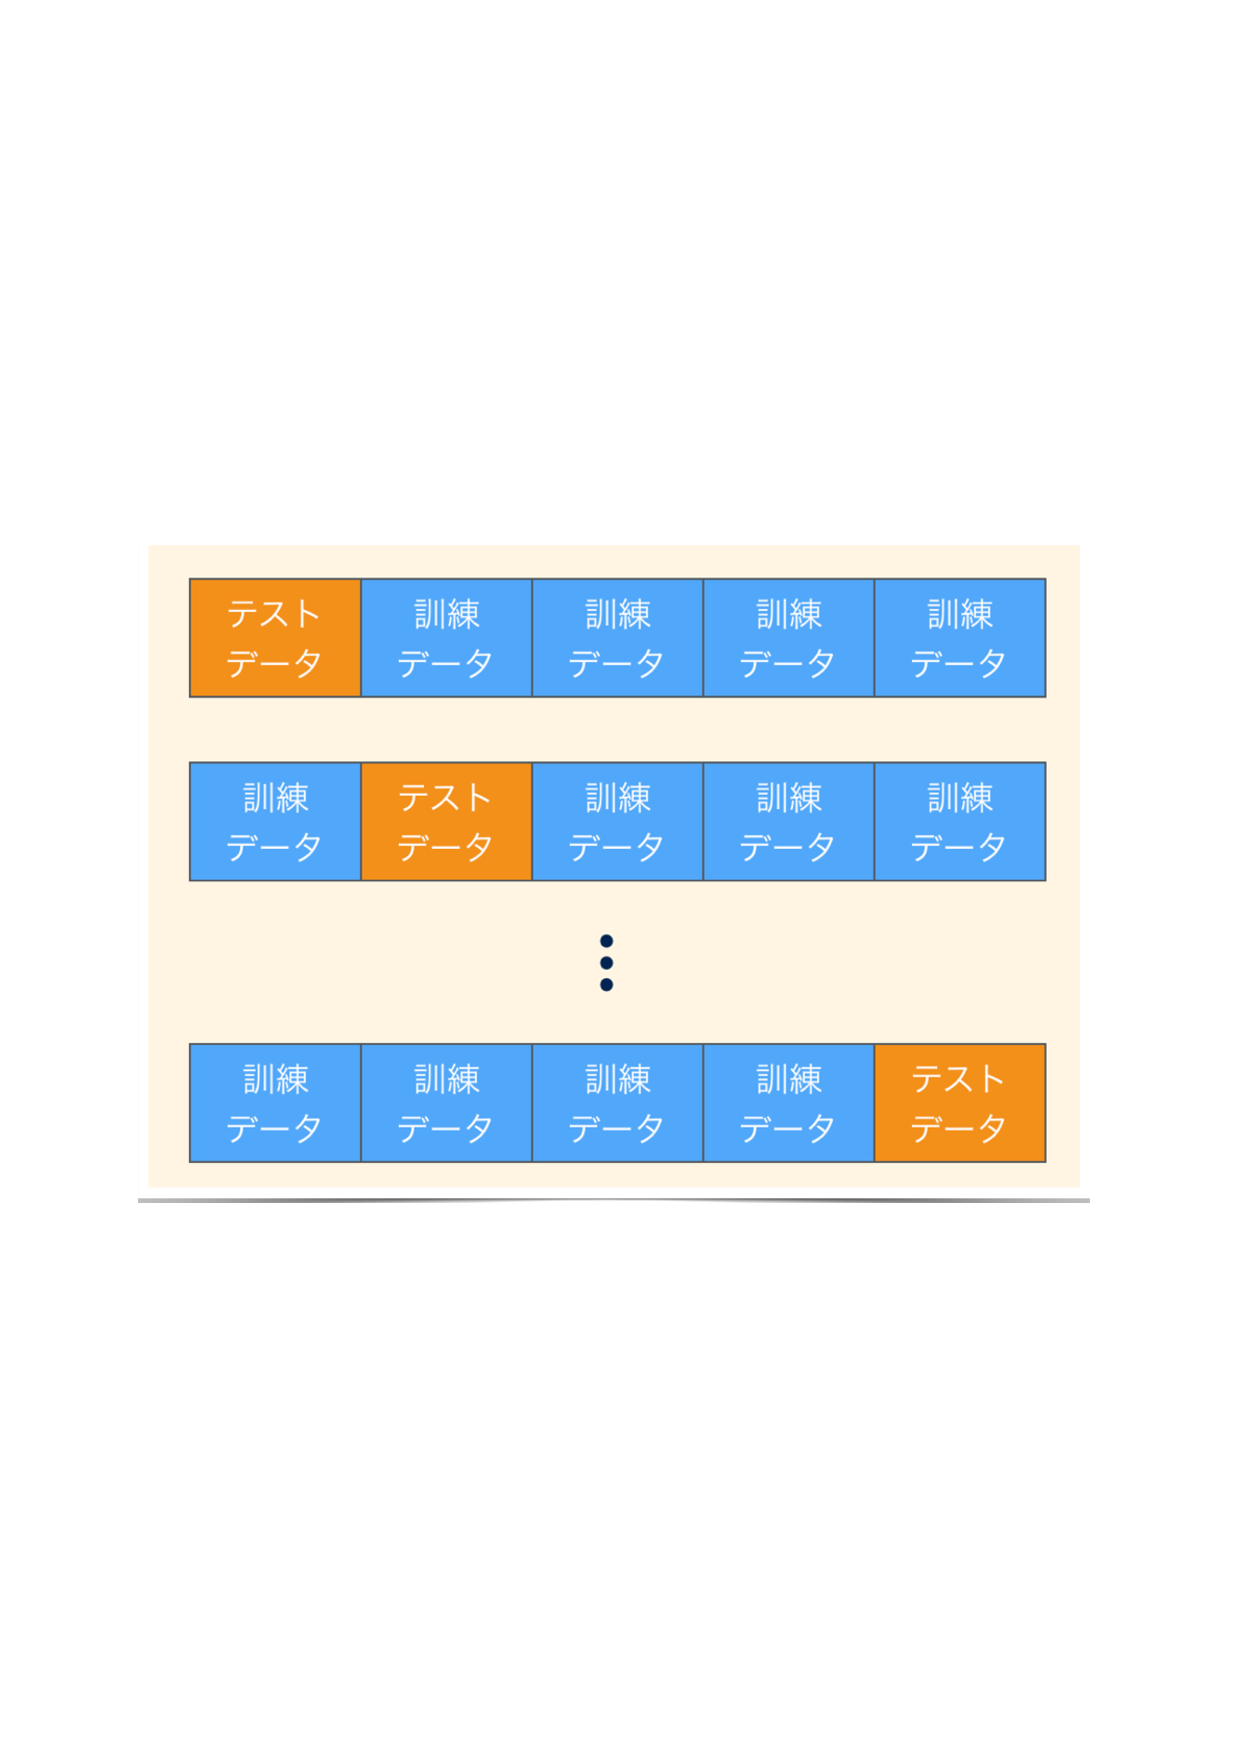
\includegraphics[keepaspectratio, scale=0.4]{./images/k-fold.pdf}
     \caption{k-分割交差検証法の例}
  \end{figure}
  \begin{itemize}
    \item テストデータと訓練データを分割して各ステップでテスト誤差を求める
    \item すべてのステップが終わった後に平均テスト誤差を求める
  \end{itemize}
\end{frame}

%-------------------

\section{推定量,バイアス,バリアンス}

%-------------------

\begin{frame}{点推定量}
  \begin{itemize}
    \item 関心のある量について\textcolor{red}{最良の}予測を1つ推定する試み
    \item パラメータ$\bm{\theta}$の点推定を$\hat{\bm{\theta}}$と表す
    \item $\{\bm{x}^{(1)} , ..., \bm{x}^{(m)}\}$を$m$個における点推定量はデータの任意の関数となる
    \begin{itemize}
      \item $\{\bm{x}^{(1)} , ..., \bm{x}^{(m)}\}$は独立同分布(i.i.d.)に従う
    \end{itemize}
  \end{itemize}
  \begin{equation}
    \hat{\bm{\theta}}_{m} = g(\bm{x}^{(1)} , ..., \bm{x}^{(m)})
  \end{equation}
  \begin{itemize}
    \item $g$が$\bm{\theta}$の真の値に近い値を返す必要はない
    \item $g$の値域が$\bm{\theta}$に許容される値の集合である必要はない
    \begin{itemize}
      \item ほとんどの関数が推定量として利用可能
      \item ただし\textcolor{red}{良い推定量}は$\bm{\theta}$の真の値に近い出力を出す関数
    \end{itemize}
    \item データは確率的な過程から抽出されるため$\hat{\bm{\theta}}$は確率変数
  \end{itemize}
\end{frame}

%-------------------

\begin{frame}{関数推定}
  \begin{itemize}
    \item 入力ベクトル$\bm{x}$に対する出力$\bm{y}$を予測
    \item $\bm{y}$と$\bm{x}$の関係を記述する関数$f(\bm{x})$が存在すると仮定
    \item よくある設定として以下の問題を考える
    \begin{itemize}
      \item $\bm{\epsilon}$は$\bm{x}$からは予測できないノイズ項
    \end{itemize}
  \end{itemize}
  \begin{equation}
    \bm{y} = f(\bm{x}) + \bm{\epsilon}
  \end{equation}
  \begin{itemize}
    \item モデルか関数推定$\hat{f}$で$f$を近似したい
    \begin{itemize}
      \item 関数推定は$\bm{\theta}$を推定するのと同じ
    \end{itemize}
  \item 関数推定量$\hat{f}$は\textcolor{red}{関数空間における点推定量}にすぎない
  \end{itemize}
\end{frame}

%-------------------

\begin{frame}{バイアス}
  \begin{itemize}
    \item 推定量のバイアスは以下のように表される
    \begin{itemize}
      \item $\mathbb{E}(\hat{\bm{\theta}}_{m})$は全データに関する期待値
      \item $\bm{\theta}$は潜在的なパラメータの真の値
    \end{itemize}
  \end{itemize}
  \begin{equation}
    bias(\hat{\bm{\theta}}_{m}) = \mathbb{E}(\hat{\bm{\theta}}_{m}) - \bm{\theta}
  \end{equation}
  \begin{itemize}
    \item $bias(\hat{\bm{\theta}}_{m}) = \bm{0}$である場合は\textcolor{red}{不偏}であるという
    \begin{itemize}
      \item $\mathbb{E}(\hat{\bm{\theta}}_{m}) = \bm{\theta}$であるのと等価
    \end{itemize}
    \item $\lim_{m \to \infty} bias(\hat{\bm{\theta}}_{m}) = 0$の場合は\textcolor{red}{漸近不偏}であるという
    \begin{itemize}
      \item $\lim_{m \to \infty} \mathbb{E}(\hat{\bm{\theta}}_{m}) = \bm{\theta}$であるのと等価
    \end{itemize}
    \item 一般的にバイアスは\textcolor{blue}{小さい}方が良いとされる
    \begin{itemize}
      \item 推定量の期待値と真の値が近いということになるため
    \end{itemize}
  \end{itemize}
\end{frame}

%-------------------

\begin{frame}{分散 , 標準誤差}
  \begin{itemize}
    \item 推定量がデータのサンプル関数としてそれだけ変化すると予想されるか
    \item 推定量の\textcolor{red}{バリアンス}とは分散$Var(\hat(\theta))$のこと
    \item 分散の平方根は\textcolor{red}{標準誤差}と呼ばれ , $SE(\hat{\theta})$と表される
    \item 推定量の分散や標準誤差はデータ集合を繰り返しサンプリングする際に推定量がどの程度変化するのかを示す尺度
    \item バイアスと同様バリアンスも\textcolor{blue}{小さい}方が好まれる
  \end{itemize}
  \begin{exampleblock}{サンプル平均の標準誤差}
    \begin{itemize}
      \item サンプル平均の標準誤差は以下のように表される
      \item $\sigma^{2}$はサンプル$x^{(i)}$の分散
    \end{itemize}
    \begin{equation}
      SE(\hat{\mu}_{m}) = \sqrt{Var \left[ \dfrac{1} {m} \sum_{i=1}^{m} x^{(i)} \right]} = \dfrac{\sigma} {\sqrt{m}}
    \end{equation}
    \begin{itemize}
      \item 真の標準誤差を過小評価してしまっている
      \begin{itemize}
        \item $m$が非常に大きい場合はこの過小評価は無視できる
      \end{itemize}
    \end{itemize}
  \end{exampleblock}
\end{frame}

%-------------------

\begin{frame}{MSEとバイアス,バリアンス}
  \begin{itemize}
    \item 大きなバイアスか大きなバリアンスをもつモデルのどちらかしか得られない場合はどのようにモデルを選択すべきか
    \begin{itemize}
      \item 交差検証
      \item \textcolor{red}{平均二乗誤差(MSE)を比較}
    \end{itemize}
    \item MSEは以下のように表すことができる
  \end{itemize}
  \begin{equation}
    MSE = \mathbb{E}[(\hat{\theta}_{m} - \theta)^{2}] = bias(\hat{\theta}_{m})^{2} + Var(\hat{\theta}_{m})^{2}
  \end{equation}
  \begin{itemize}
    \item MSEの評価にはバイアスとバリアンスの両方が組み込まれてる
    \item 望ましい推定量は以下のような推定量である
    \begin{itemize}
      \item MSEを小さくする
      \item バイアスとバリアンスをある程度抑えている
    \end{itemize}
  \end{itemize}
\end{frame}

%-------------------

\begin{frame}{バイアス , バリアンスの関係}
  \begin{figure}[htbp]
    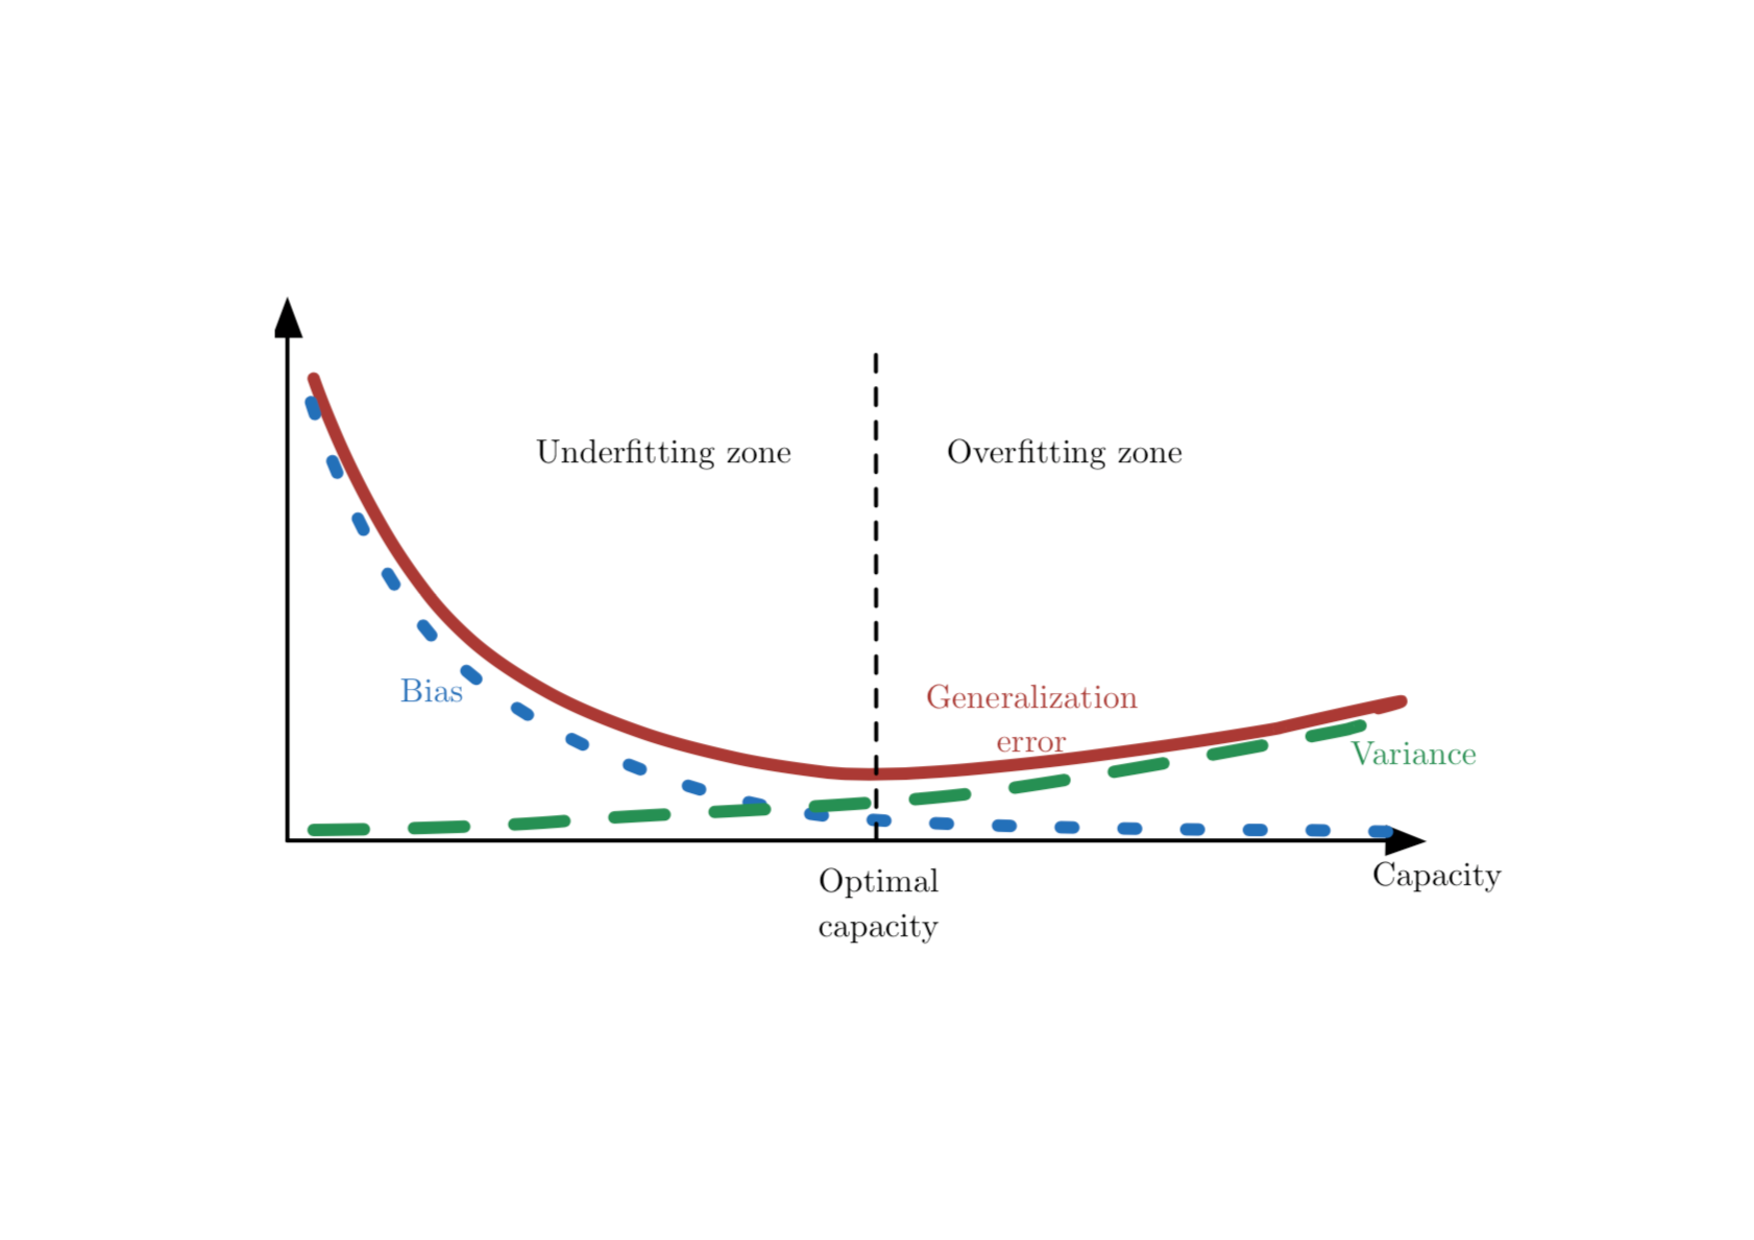
\includegraphics[keepaspectratio, scale=0.4, angle=-90]{./images/bias-variance.pdf}
    \caption{バイアス , バリアンスの関係.青点線がバイアス , 緑点線がバリアンス , 赤線がテスト誤差 , 黒点線が最適な容量の位置}
  \end{figure}
  \begin{itemize}
    \item バイアスとバリアンスの関係は過学習 , 未学習と密接に関係している
    \item 容量を増加させるごとにバイアスが減少し , バリアンスが増加する
  \end{itemize}
\end{frame}

%-------------------

\begin{frame}{一致性}
  \begin{itemize}
    \item これまで訓練データ量が固定の場合を見てきた
    \item \textcolor{red}{訓練データの量が増える場合}の推定量の挙動
    \item 具体的には以下のようになってほしい
  \end{itemize}
  \begin{equation}
    \lim_{m \to \infty} \hat{\theta}_{m} = \theta
  \end{equation}
  \begin{itemize}
    \item このような条件のことを\textcolor{red}{一致性}と呼ぶ
    \item 一致性によってデータ数が増えるとバイアスが減少することが保証される
    \begin{itemize}
      \item その逆は真ではない
      \item 漸近的に不偏であることは一致性を意味しない
    \end{itemize}
  \end{itemize}
\end{frame}

%-------------------

\end{document}

